\documentclass[12pt, spanish]{article}
\usepackage[spanish]{babel}
\selectlanguage{spanish}
%\usepackage{natbib}
\usepackage{url}
\usepackage[utf8x]{inputenc}
\usepackage{graphicx}
\graphicspath{{images/}}
\usepackage{parskip}
\usepackage{fancyhdr}
\usepackage{vmargin}
\usepackage{multirow}
\usepackage{float}
\usepackage{chngpage}

\usepackage{amsfonts}

\usepackage{subcaption}

\usepackage{hyperref}
\usepackage[
    type={CC},
    modifier={by-nc-sa},
    version={4.0},
]{doclicense}

\hypersetup{
    colorlinks=true,
    linkcolor=blue,
    filecolor=magenta,
    urlcolor=cyan,
}

% para codigo
\usepackage{listings}
\usepackage{xcolor}



%% configuración de listings

\definecolor{listing-background}{HTML}{F7F7F7}
\definecolor{listing-rule}{HTML}{B3B2B3}
\definecolor{listing-numbers}{HTML}{B3B2B3}
\definecolor{listing-text-color}{HTML}{000000}
\definecolor{listing-keyword}{HTML}{435489}
\definecolor{listing-identifier}{HTML}{435489}
\definecolor{listing-string}{HTML}{00999A}
\definecolor{listing-comment}{HTML}{8E8E8E}
\definecolor{listing-javadoc-comment}{HTML}{006CA9}

\lstdefinestyle{eisvogel_listing_style}{
  language         = python,
%$if(listings-disable-line-numbers)$
%  xleftmargin      = 0.6em,
%  framexleftmargin = 0.4em,
%$else$
  numbers          = left,
  xleftmargin      = 0em,
 framexleftmargin = 0em,
%$endif$
  backgroundcolor  = \color{listing-background},
  basicstyle       = \color{listing-text-color}\small\ttfamily{}\linespread{1.15}, % print whole listing small
  breaklines       = true,
  frame            = single,
  framesep         = 0.19em,
  rulecolor        = \color{listing-rule},
  frameround       = ffff,
  tabsize          = 4,
  numberstyle      = \color{listing-numbers},
  aboveskip        = 1.0em,
  belowskip        = 0.1em,
  abovecaptionskip = 0em,
  belowcaptionskip = 1.0em,
  keywordstyle     = \color{listing-keyword}\bfseries,
  classoffset      = 0,
  sensitive        = true,
  identifierstyle  = \color{listing-identifier},
  commentstyle     = \color{listing-comment},
  morecomment      = [s][\color{listing-javadoc-comment}]{/**}{*/},
  stringstyle      = \color{listing-string},
  showstringspaces = false,
  escapeinside     = {/*@}{@*/}, % Allow LaTeX inside these special comments
  literate         =
  {á}{{\'a}}1 {é}{{\'e}}1 {í}{{\'i}}1 {ó}{{\'o}}1 {ú}{{\'u}}1
  {Á}{{\'A}}1 {É}{{\'E}}1 {Í}{{\'I}}1 {Ó}{{\'O}}1 {Ú}{{\'U}}1
  {à}{{\`a}}1 {è}{{\'e}}1 {ì}{{\`i}}1 {ò}{{\`o}}1 {ù}{{\`u}}1
  {À}{{\`A}}1 {È}{{\'E}}1 {Ì}{{\`I}}1 {Ò}{{\`O}}1 {Ù}{{\`U}}1
  {ä}{{\"a}}1 {ë}{{\"e}}1 {ï}{{\"i}}1 {ö}{{\"o}}1 {ü}{{\"u}}1
  {Ä}{{\"A}}1 {Ë}{{\"E}}1 {Ï}{{\"I}}1 {Ö}{{\"O}}1 {Ü}{{\"U}}1
  {â}{{\^a}}1 {ê}{{\^e}}1 {î}{{\^i}}1 {ô}{{\^o}}1 {û}{{\^u}}1
  {Â}{{\^A}}1 {Ê}{{\^E}}1 {Î}{{\^I}}1 {Ô}{{\^O}}1 {Û}{{\^U}}1
  {œ}{{\oe}}1 {Œ}{{\OE}}1 {æ}{{\ae}}1 {Æ}{{\AE}}1 {ß}{{\ss}}1
  {ç}{{\c c}}1 {Ç}{{\c C}}1 {ø}{{\o}}1 {å}{{\r a}}1 {Å}{{\r A}}1
  {€}{{\EUR}}1 {£}{{\pounds}}1 {«}{{\guillemotleft}}1
  {»}{{\guillemotright}}1 {ñ}{{\~n}}1 {Ñ}{{\~N}}1 {¿}{{?`}}1
  {…}{{\ldots}}1 {≥}{{>=}}1 {≤}{{<=}}1 {„}{{\glqq}}1 {“}{{\grqq}}1
  {”}{{''}}1
}
\lstset{style=eisvogel_listing_style}


\usepackage[default]{sourcesanspro}

\setmarginsrb{2 cm}{1 cm}{2 cm}{2 cm}{1 cm}{1.5 cm}{1 cm}{1.5 cm}

\title{Práctica 0:\\
Introducción a OpenCV  \hspace{0.05cm} }
\author{Antonio David Villegas Yeguas}
\date{\today}

\renewcommand*\contentsname{hola}

\makeatletter
\let\thetitle\@title
\let\theauthor\@author
\let\thedate\@date
\makeatother

\pagestyle{fancy}
\fancyhf{}
\rhead{\theauthor}
\lhead{\thetitle}
\cfoot{\thepage}

\begin{document}

%%%%%%%%%%%%%%%%%%%%%%%%%%%%%%%%%%%%%%%%%%%%%%%%%%%%%%%%%%%%%%%%%%%%%%%%%%%%%%%%%%%%%%%%%

\begin{titlepage}
    \centering
    \vspace*{0.3 cm}
    
\includegraphics[scale = 0.50]{ugr.png}\\[0.7 cm]
    %\textsc{\LARGE Universidad de Granada}\\[2.0 cm]
    \textsc{\large 4º CSI 2020/21 - Grupo 2}\\[0.5 cm]
    \textsc{\large Grado en Ingeniería Informática}\\[0.5 cm]
    \rule{\linewidth}{0.2 mm} \\[0.2 cm]
    { \huge \bfseries \thetitle}\\
    \rule{\linewidth}{0.2 mm} \\[1 cm]

    \begin{minipage}{0.4\textwidth}
        \begin{flushleft} \large
            \emph{Autor:}\\
            \theauthor\\
			 \emph{DNI:}\\
            77021623-M
            \end{flushleft}
            \end{minipage}~
            \begin{minipage}{0.4\textwidth}
            \begin{flushright} \large
            \emph{Asignatura: \\
            Visión por Computador}   \\
            \emph{Correo:}\\
            advy99@correo.ugr.es
        \end{flushright}
    \end{minipage}\\[0.5cm]

    {\large \thedate}\\[0.5cm]
    %{\url{https://github.com/advy99/AA/}}
    {\doclicenseThis}

    \vfill

\end{titlepage}

%%%%%%%%%%%%%%%%%%%%%%%%%%%%%%%%%%%%%%%%%%%%%%%%%%%%%%%%%%%%%%%%%%%%%%%%%%%%%%%%%%%%%%%%%

\tableofcontents
\pagebreak

%%%%%%%%%%%%%%%%%%%%%%%%%%%%%%%%%%%%%%%%%%%%%%%%%%%%%%%%%%%%%%%%%%%%%%%%%%%%%%%%%%%%%%%%%


\section*{Introducción}

Esta práctica trata sobre el uso de las herramientas que utilizaremos a lo largo del curso para el desarrollo de la asignatura, en concreto Python, OpenCV y la plataforma Colab principalmente, aunque nos apoyaremos en otras bibliotecas como NumPy, MatPlotLib, entre otras.

En esta práctica de introducción se nos plantean cinco ejercicios que debemos resolver haciendo uso de estas herramientas y comprobar que funcionan correctamente tanto en nuestros entornos locales como en la plataforma Colab.


En este documento se encuentran las explicaciones de que se ha hecho y el por qué, pero no se apoyarán en el código a no ser que sea estrictamente necesario. Todo el código se encuentra disponible en el fichero \texttt{p0.py}.

\newpage

\section{Ejercicio 1}

\textbf{\large Enunciado: Escribir una función que lea el fichero de una imagen permita mostrarla tanto en grises como en color (\texttt{im=leeimagen(filename, flagColor)})}


Para este ejercicio simplemente he implementado la función \texttt{leeimagen}, que pasando una ruta de un fichero lee la imagen utilizando OpenCV, y como segundo parámetro tiene el modo de lectura del color, para este segundo parámetro utilizaremos 0 para leer en blanco y negro y 1 para leer a color, aunque hay disponibles más opciones \cite{read_image_opencv}

Además he creado otra función para visualizar las imágenes de forma que siempre que visualice algo a lo largo de la práctica, utilizaré esta función.

Esta función \texttt{muestra\_imagen} recibe una imagen (una matriz) y opcionalmente un título. Mostrará la imagen en una ventana de MatPlotLib con el titulo dado. Esta función comprobará si la imagen es monobanda o tribanda para saber la forma correcta de visualización y si ha de invertir los colores en el caso tribanda, ya que MatPlotLib utiliza el sistema RBG, sin embargo OpenCV lee las imágenes como BGR\cite{BGR_cv}. He decidido utilizar MatPlotLib ya que, aunque hay que invertir los canales, OpenCV da problemas para su ejecución en Colab.

\section{Ejercicio 2}

\textbf{\large Enunciado: Escribir una función que visualice una matriz de números reales cualquiera ya sea monobanda o tribanda (\texttt{pintaI(im)}). Para ello deberá de trasladar y escalar el rango de cada banda al intervalo [0,1] sin pérdida de información.}

De cara a este ejercicio he realizado dos funciones:

\begin{enumerate}
	\item \texttt{normalizar\_imagen}: Recibe una imagen. Devuelve una imagen normalizada, es decir, escalada al rango [0,1], con tres bandas y sin perdida de información.
	\item \texttt{pintaI}: Normaliza una imagen utilizando la función anterior y la muestra por pantalla.
\end{enumerate}

He realizado la primera función ya que nos será útil al trabajar que todas las imágenes tengan el mismo formato de cara a los próximos ejercicios.

Para normalizar la imagen, he buscado el valor máximo y mínimo de la matriz utilizando \texttt{np.min} y \texttt{np.max}\cite{np_min_max}, tras esto he desplazado la matriz para que el valor más pequeño este en el 0, de forma que no perdamos información:

$$ imagen = imagen - valor\_minimo $$

De esta forma, si el valor más pequeño era negativo, se ha sumado hasta llegar a cero, y si es positivo se ha restado, siendo en todo caso cero el nuevo valor.

Tras esto he divido todos los valores por el valor máximo. Este valor máximo también se ha visto desplazado, luego lo tenemos que tener en cuenta.

$$ imagen = imagen / (maximo - minimo) $$

O lo que es equivalente a estas dos operaciones:

$$ imagen = (imagen - minimo) / (maximo - minimo) $$

Otra cosa que he tenido en cuenta es que si el máximo menos el mínimo vale 0, es imposible dividir. En ese caso la imagen es toda de un único color, y como no sabemos en que rango se encontraba he supuesto que es una imagen en negro, y la imagen entera se sustituye por una matriz de unos utilizando \texttt{np.ones}\cite{np_ones}.

De cara a próximos ejercicios he añadido una comprobación de que si la imagen es monobanda se convierte a tribanda triplicando la única banda existente, de esta forma se mantiene la información (los colores son equivalentes al tener el mismo valor tanto en la capa R como en la G y en la B), mientras que podremos realizar operaciones de forma más fácil en los siguientes ejercicios.


He decidido escoger el máximo y el mínimo de todas las bandas y escalarlo todo usando esos valores ya que si por algún motivo la imagen en una de las bandas no utiliza el valor más alto perderíamos información, por ejemplo, si las bandas van de 0 a 255, pero el valor más alto de azul es 170, si normalizamos la banda azul a 170 en lugar de 255 estamos añadiendo una información de un azul más intenso que antes no existía.

La segunda función, \texttt{pintaI}, recibe una imagen por parámetro, la cual es normalizada con la función anterior, y muestra por pantalla la imagen normalizada utilizando la función para mostrar imágenes del ejercicio 1.

Para comprobar el funcionamiento he creado dos matrices (una monobanda y otra tribanda) de tamaño 500 por 500 con valores aleatorios obtenidos de una distribución uniforme entre 0 y 1 utilizando el método \texttt{np.random.randn}\cite{np_randn} pero los he multiplicado por 5 para comprobar que mi función es correcta. Estas son las visualizaciones del resultado:

\begin{figure}[H]
	\centering
	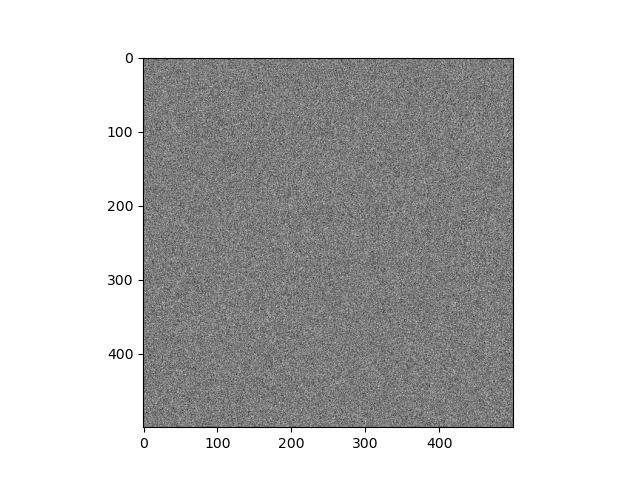
\includegraphics[scale = 0.70]{monobanda.png}
	\caption{Imagen obtenida de la matriz monobanda.}
	\label{fig:ej2-mono}
	
\end{figure}


\begin{figure}[H]
	\centering
	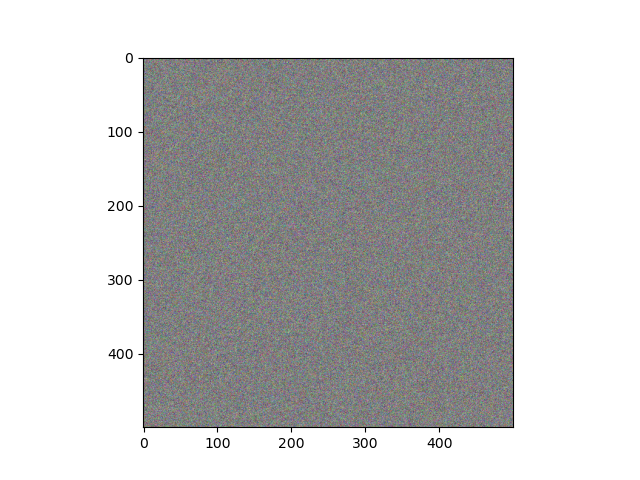
\includegraphics[scale = 0.70]{tribanda.png}
	\caption{Imagen obtenida de la matriz tribanda.}
	\label{fig:ej2-tri}
	
\end{figure}

Como vemos, en la imagen monobanda solo observamos tonalidades grises, mientras que en la tribanda si encontramos píxeles de colores.

Además, he aplicado la función a una imagen ya dada para comprobar que sigue visualizando de forma correcta las imágenes.

\begin{figure}[H]
	\centering
	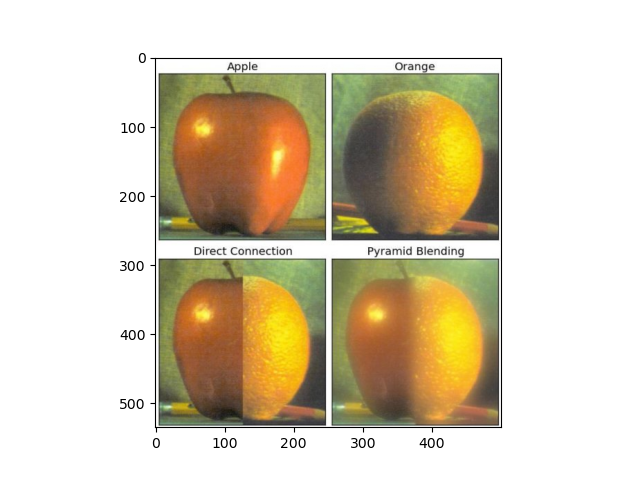
\includegraphics[scale = 0.70]{ej2-orig.png}
	\caption{Imagen obtenida de la imagen original.}
	\label{fig:ej2-tri}
	
\end{figure}

\section{Ejercicio 3}

\textbf{\large Escribir una función que visualice varias imágenes a la vez(fusionando las imágenes en una última imagen final): \texttt{pintaMI(vim)} (vim será una secuencia de imágenes) ¿Qué pasa si las imágenes no son todas del mismo tipo(nivel de gris, color, blanco-negro)?.}

A la pregunta de como evitar el problema de si son imágenes a color o en blanco y negro (tribanda o monobanda), y si utilizan distintos niveles de gris o de colores, la respuesta es la función que hemos realizado en el ejercicio 2. Aprovechando que nos pedían normalizar las imágenes a un rango de 0 y 1, y con el añadido de pasar toda imagen a tribanda, no tendremos problemas a la hora de apilar las matrices.

El único problema encontrado es como apilar matrices de distintas dimensiones, que lo resolveremos con la primera de las funciones.

De cara a este ejercicio he realizado dos funciones:

\begin{enumerate}
	\item \texttt{une\_imagenes}: Recibe una lista de imágenes. Devuelve una imagen con todas las imágenes concatenadas.
	\item \texttt{pintaMI}: Visualiza una lista de imágenes como una única imagen.
\end{enumerate}

La primera función, dada una lista de imágenes, las apila en una única imagen final utilizando el método \texttt{np.hstack}\cite{hstack} de NumPy. De cara a utilizar esta función encontramos dos problemas:

\begin{enumerate}
	\item Imágenes no normalizadas: Lo resolveremos aplicando la función desarrollada en el ejercicio 2 a cada imagen de la lista.
	\item Distintas dimensiones de las imágenes: Resolveremos este problema buscando la imagen con mayor altura, y añadiendo una franja negra a todas las imágenes de menor altura, de forma que todas las imágenes tengan el mismo numero de filas para poder aplicar la operación. Al unir las imágenes de forma horizontal, solamente es necesario que tengan mismo número de filas, mientras que el número de columnas es indiferente.
\end{enumerate}

Tras añadir la franja negra y unir las imágenes, este es el resultado:

\begin{figure}[H]
	\centering
	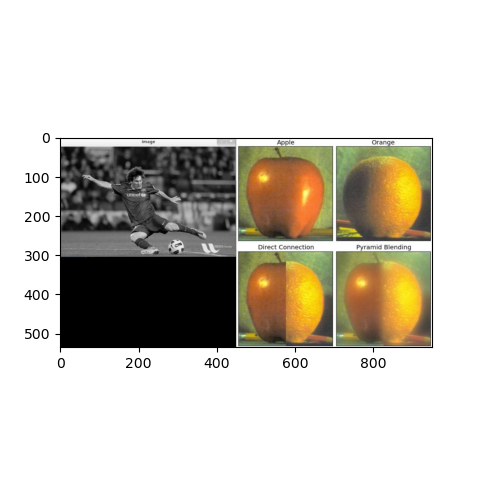
\includegraphics[scale = 1]{union.png}
	\caption{Imagen obtenida de la unión de dos imágenes.}
	\label{fig:ej3}
	
\end{figure}

\newpage

\section{Ejercicio 4}

\textbf{\large Escribir unafunción que modifique el coloren la imagen de cada uno de los elementos de una lista de coordenadas de píxeles. (Recordarque (fila, columna) es lo contrario a (x,y). Es decir fila=y, columna=x).}

Para este ejercicio he escrito una función \texttt{modifica\_color}, que recibe como parámetros una imagen, una lista con parejas de enteros como coordenadas, que serán las coordenadas de la imagen a modificar el color, y por último una tupla de tres elementos en el rango [0,1] que conformarán el nuevo color en formato BGR.

La única consideración a tener en cuenta es que en este caso, a la hora de modificar el color, si nos referimos a la fila \texttt{a} y columna \texttt{b}, en la imagen las coordenadas están invertidas, luego hay que modificar la posición \texttt{(b,a)}.

Para probar esta función he rellenado una lista con las coordenadas de un cuadrado de tamaño 50x50 y he seleccionado como color un rosa pastel.

Tras modificar el color de la sección de la imagen, este es el resultado:

\begin{figure}[H]
	\centering
	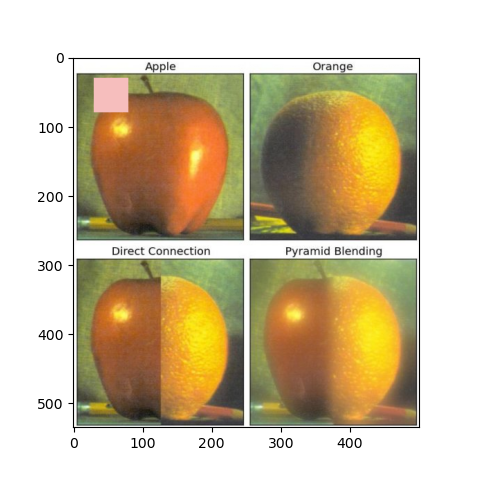
\includegraphics[scale = 1]{color.png}
	\caption{Imagen obtenida de la modificación del color de parte de la imagen.}
	\label{fig:ej4}
	
\end{figure}

\newpage

\section{Ejercicio 5}

\textbf{\large Una función que sea capaz de representar varias imágenes con sus títulos en una misma ventana.}

Para este ejercicio he utilizado la función \texttt{une\_imagenes} del ejercicio 3, y he modificado la función \texttt{mostrar\_imagen} del ejercicio 1, añadiendo un parámetro por defecto vacío que sera una cadena de texto que funcionará como título de la ventana.

Tras estas modificaciones, este es el resultado: 

\begin{figure}[H]
	\centering
	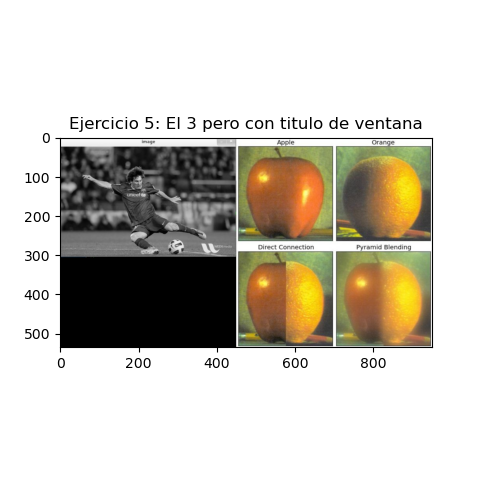
\includegraphics[scale = 1]{union_titulo.png}
	\caption{Imagen obtenida de la unión de dos imágenes y visualizada con un título.}
	\label{fig:ej5}
	
\end{figure}

\newpage

\section{Ejecución en Colab}

De cara a la ejecución en Colab simplemente tenemos que descomentar las dos lineas que activan la sincronización con Google Drive:

\begin{lstlisting}
from google.colab import drive
drive.mount("/content/drive")
\end{lstlisting}

Y además, completar la ruta de las imágenes en nuestro disco de Drive. Por defecto la variable estará vacía para la ejecución en nuestro entorno:

\begin{lstlisting}
RUTA_DRIVE=""
\end{lstlisting}

Simplemente tenemos que completar la ruta acabando en / y sin incluir la carpeta imagenes, por ejemplo:

\begin{lstlisting}
# si las imagenes estan en la raiz de tu drive, dentro de imagenes/
RUTA_DRIVE="./drive/My Drive/"
\end{lstlisting}

Tras esto, podemos ejecutar todo el script proporcionado en el fichero de python adjunto en la entrega.

\newpage

\section{Referencias, material y documentación usada}


\begin{thebibliography}{9}

\bibitem{read_image_opencv}
Flags lectura de imágenes en OpenCV - Documentación oficial de OpenCV

\url{https://docs.opencv.org/4.4.0/d4/da8/group__imgcodecs.html}

\bibitem{BGR_cv}
Lectura de imágenes en OpenCV - imread - Documentación oficial de OpenCV

\url{https://docs.opencv.org/4.4.0/d4/da8/group__imgcodecs.html#ga288b8b3da0892bd651fce07b3bbd3a56}

\bibitem{np_min_max}
Mínimo y máximo de una estructura de NumPy - Documentación oficial de NumPy

\url{https://numpy.org/doc/stable/reference/generated/numpy.ndarray.min.html}
\url{https://numpy.org/doc/stable/reference/generated/numpy.ndarray.max.html}

\bibitem{np_ones}
Array de unos en NumPy - Documentación oficial de NumPy

\url{https://numpy.org/doc/stable/reference/generated/numpy.ones.html}

\bibitem{np_randn}
Estructura con valores aleatorios entre 0 y 1 obtenidos a partir de una distribución uniforme - Documentación oficial de NumPy.

\url{https://numpy.org/doc/stable/reference/random/generated/numpy.random.randn.html}

\bibitem{hstack}
Apilar dos matrices de forma horizontal - Documentación oficial de NumPy

\url{https://numpy.org/doc/stable/reference/generated/numpy.hstack.html}

\bibitem{vstack}
Apilar dos matrices de forma vertical - Documentación oficial de NumPy

\url{https://numpy.org/doc/stable/reference/generated/numpy.vstack.html}

\end{thebibliography}

\end{document}
